%!TEX root = ../main.tex
%%=====================================================================
%%  APPENDIX
%%
%%  WHAT STAYS HERE, now that §4 exists:
%%   A.1  full per-configuration results, both trading layers, with seed
%%        standard deviations and era breakdowns
%%   A.2  the twelve methods in detail (moved out of §3)
%%   A.3  the aggregation identity with its derivation and reconstruction
%%        error
%%   A.4  the Monte Carlo size table for the spanning statistics
%%   A.5  the stacked-factor experiment, if included at all
%%   A.6  implementation and replication: the validity screen, the seed
%%        protocol, the note that the hardware is non-deterministic so
%%        exact reproduction is bounded at |dSR| <= 0.08, and THE TWO
%%        SHARPE CONVENTIONS with a conversion note
%%
%%  WHAT MOVED OUT, to §4: the two standard errors and their derivation,
%%  the rho^2 correction, the reliability calculation, the calibrated
%%  simulation. Those are the paper's econometrics and they belong in the
%%  body.
%%
%%  FRONT MATTER THE AUTHORS MUST SUPPLY:
%%   * Yixuan He's affiliation -- nothing in the repository states it
%%   * Lunji Zhu's email
%%   * any grant or data acknowledgement, or none
%%=====================================================================
\section{Appendix: Data, Implementation, and Additional Results}
\label{app:supp}

This appendix has two parts. \appref{app:rules} to \appref{app:calendar} give the construction of each clusterizer, the treatment of degenerate groups, the realized partition sizes, the trading head's architecture and schedule, the identifiers under which every arm was run, the sweep over the number of groups, and the calendar offset between the panel and the factor file. \appref{app:dose} to \appref{app:costs} give the additional results the text refers to, in the order in which the text refers to them: an experiment that degrades a real partition continuously toward a random one, the mechanism behind the estimation-window effect, three robustness checks on the factor and peer comparisons, and the transaction-cost calculation in full. Data and code are submitted with the replication files.

\subsection{The Clusterizers in Detail}
\label{app:rules}

All clusterizers receive the same input: the day's universe of $\N_t$ stocks
(\secref{sec:panel}) and the trailing window of market residuals
$\mathbf{R}_{\mathrm{tr}} \in \real^{60 \times \N_t}$, 60 days ending
at $t$. All target $\K = 30$ groups. Where a correlation matrix appears
it is $\Cmat = \operatorname{corr}(\mathbf{R}_{\mathrm{tr}})$, the
$\N_t \times \N_t$ sample correlation of the window's columns.

\paragraph{$k$-means on returns.} Each stock is treated as the point of
its own 60 residual returns in $\real^{60}$, and $k$-means with
Euclidean distance partitions those points ($30$ clusters, $4$
restarts). No correlation matrix is formed. Because the coordinates are
unstandardized, distance is dominated by volatility. High-volatility names sit far from everything and often become singletons (about 10 a
day), whose members the trading stage later drops (\tabref{tab:methods}, note b).

\paragraph{Average and complete linkage.} Agglomerative clustering on
the dissimilarity $\Dmat = 1 - \Cmat$: start from singletons and
repeatedly merge the two closest clusters until 30 remain. The two
clusterizers differ only in how the distance between clusters is defined: the
average of all cross-pair dissimilarities, or the maximum. Both are deterministic, so the same input gives the same partition and
there is no seed to vary.

\paragraph{Spectral, unsigned.} Spectral clustering on the affinity
$|\Cmat|$: eigenvectors of the graph Laplacian of $|\Cmat|$ embed the
stocks, and $k$-means groups the embedded points. Taking absolute
values means a strong negative correlation counts as a strong link.

\paragraph{PCA loadings.} The 10 leading eigenvectors of $\Cmat$
give each stock a 10-dimensional coordinate, its loadings on the top
10 principal components, and $k$-means groups those coordinates. Stocks
are grouped by which factors they load on.

\paragraph{\textsc{sponge}.} \citet{cucuringu2019sponge} give two
variants. We use the symmetric one, \textsc{sponge}$_{\mathrm{sym}}$,
and \textsc{sponge} in this paper always means that variant. The
correlation matrix is split into its positive part
$\Cmat^{+} = \max(\Cmat, 0)$ and negative part
$\Cmat^{-} = \max(-\Cmat, 0)$, and the method
solves a generalized eigenproblem on the two signed-graph Laplacians
(both regularization parameters set to $1$), seeking groups with
positive correlation inside and negative correlation across.
$k$-means on the resulting embedding gives the labels. Unlike in the unsigned spectral clusterizer, the sign of a correlation
is information here. A
post-processing step reassigns members of groups smaller than two to
their most correlated group. 

\paragraph{\textsc{sssnet}.} \textsc{sssnet} is the signed-graph neural
network of \citet{he2022sssnet}, trained on a clustering objective. The signed graph is
built from the same 60-day correlation matrix, node features are the
identity, and training is warm-started from a \textsc{sponge}
partition. In its original form it computes its partition at run time from a random-number stream shared with the trading head.\label{app:sssnet} In this paper it is run once, with daily seeds, to produce a fixed set of daily partitions for the whole sample, 23 July 1993 to 30 December 2024, which the five head seeds then share, exactly as for the other eight stochastic clusterizers; its partitions under seeds $1$ to $5$ are generated the same way. Across the five partition draws the rule-based book moves by $0.15$ in Sharpe ratio and the trained book at head seed $42$ by $0.13$ ($2.398$ to $2.527$), the fifth-largest and the smallest ranges among the nine stochastic clusterizers (\secref{sec:pseed}).

\paragraph{The trading-driven family.} Four clusterizers replace the
clustering criterion with a trading objective: a soft assignment matrix
over $\K$ groups is optimized directly against the payoff of the rule-based book that the
assignment would produce, then hardened by argmax. The objective is
evaluated on the trailing $252$ trading days of residuals ending the
day before the partition is applied, so no return from that day
onward enters the partition. All four warm-start from a \textsc{sponge} partition, balance
group sizes by a Sinkhorn step, and penalize groups whose members are
too weakly correlated (a cohesion floor). The four
differ in the objective and in the parameterization:
\emph{Sharpe} maximizes the plain Sharpe ratio of the induced book;
\emph{Sortino} replaces the standard deviation in that objective with
the downside deviation;
\emph{Sharpe (EW)} is a variant of \emph{Sharpe} that weights
recent days exponentially (decay $0.99$ over a $252$-day window, so the
oldest day carries $8\%$ of the newest day's weight) and differs from \emph{Sharpe} in more than the weighting (\tabref{tab:methods}, note d);
\emph{Sharpe (graph)} produces the assignment with a signed-graph network rather than free logits, and evaluates the objective on the
30-day horizon the trading signal uses.

\paragraph{\textsc{gics}.} A static sector table, from a single S\&P
1500 snapshot: no return data is read at all. The table covers $54\%$ to $73\%$ of the universe depending on the era. The remaining
names, about $35\%$ of the book on a given day, are
assigned to the group with which they correlate most strongly, so
the traded arm is a taxonomy--correlation hybrid. Its realized number
of groups is the number of sectors in the snapshot, exactly 10 on every
day of the sample, not $\K$. The snapshot predates the separation of
real estate into an eleventh sector in 2016.

\paragraph{The two controls.} $\K=1$ places every stock in one group.
Random draws each stock's label uniformly from the 30 groups,
independently each day, reading nothing.

%%  All constructions read from source this session:
%%  gen_daily_partitions.py:102-134 (kmeans/random/spectral/agglo/pca,
%%  sponge_labels), variant_f_v2a_clusterizer.py (SPONGE_sym call,
%%  _fix_tiny_clusters, fv2a machinery), tier2/work/*/work.py (the four
%%  trading-driven variants), the executed sssnet working copies.
%%  ⚠ he2022sssnet must exist in refs.bib -- check before shipping.
%%  ⚠ "about eleven" for GICS = measured 10.9; "about ten" singletons =
%%  10.3; both audited 2026-08-16.

\subsection{Two Policies for Degenerate Clusters}
\label{app:singleton}

The pipeline treats clusters of fewer than two members in two ways,
and which treatment an arm receives depends only on which code generated its partition. \textsc{sponge}'s generation path repairs them:
each orphaned member is merged into its most correlated group, and
the stock stays in the book. The Sharpe and Sortino clusterizers inherit the
same repair. Every other clusterizer passes its labels on unrepaired, and
the trading stage then deletes every member of a sub-minimum cluster
from that day's book.

The asymmetry is nominal for 11 arms and material for one. Where
the repair applies it has almost nothing to repair ($0.13$
groups per day for \textsc{sponge}, a handful of days in the whole
sample for the other two), and every clusterizer except $k$-means on returns
produces at most $0.6$ singletons per day. $k$-means on returns produces $9.8$ singleton labels per day, which the trading stage deletes as $8.65$ names per day, and at the trained component its traded book holds $491.3$ names against $499.5$ to
$500.0$ for every other arm.

The cost of the asymmetry is measured; on this panel it is too small to resolve. A second arm trades the same $k$-means partitions with singleton members merged rather than deleted, which is $k$-means under
\textsc{sponge}'s policy. That arm earns $0.04$ less in Sharpe ratio on the five-seed average and runs $0.05$ percentage points more volatile. Neither difference survives its own dispersion: the Sharpe gap carries $t=-0.9$ on four degrees of freedom and changes sign across the five seeds, and the volatility gap runs from $-0.00$ to $+0.24$ across them.
Set against $k$-means' own head-seed standard deviation of $0.112$,
the gap between the two arms sits inside the noise of a single arm's refit. Harmonizing the policy in either direction would
therefore move the leading clusterizer by less than its run-to-run noise, and
imposing the deletion policy on \textsc{sponge} would in addition rebuild every one of its partitions to change $0.0$ names per day. The repair can also empty a label, so \textsc{sponge} realizes $29.9$ clusters per day against a nominal $30$, as does \textsc{sssnet}, whose partition is warm-started from a \textsc{sponge} partition; no other data-driven arm falls short of its nominal $\K$. We keep each clusterizer's own policy and state it.

\subsection{Partition Size Distributions}
\label{app:sizes}

Nominally every arm but \textsc{gics} and the $\K=1$ control targets
$\K = 30$. In realized terms they differ widely (\tabref{tab:sizes}), and the
differences do not track
performance: over the 12
clusterizers, the Spearman correlation between effective $\K$ and the mean-of-per-seed Sharpe ratio is $-0.15$ with $p = 0.63$.

\begin{table}[htbp]
\centering
\caption{Realized partition shape, mean over all $6{,}913$ out-of-sample days}
\label{tab:sizes}
\begin{threeparttable}
\small
\begin{tabular}{@{}lrrrr@{}}
\toprule
Arm & Effective $\K$ & Largest group & Singletons/day & Groups $<5$/day \\
\midrule
Sharpe (EW)          & $29.26$ & $22.1$  & $0.00$ & $0.07$ \\
Sortino              & $29.08$ & $23.1$  & $0.00$ & $0.06$ \\
Sharpe               & $28.98$ & $23.5$  & $0.00$ & $0.08$ \\
Sharpe (graph) & $28.58$ & $24.9$ & $0.01$ & $0.06$ \\
Random & $28.36$ & $25.5$  & $0.00$ & $0.01$ \\
PCA loadings & $26.86$ & $30.9$ & $0.01$ & $0.12$ \\
Spectral (unsigned) & $23.83$ & $40.7$ & $0.01$ & $0.95$ \\
\textsc{sponge} & $23.54$ & $40.7$ & $0.00$ & $1.30$ \\
\textsc{sssnet} & $22.36$ & $40.8$ & $0.00$ & $1.81$ \\
Complete linkage & $22.25$ & $49.8$ & $0.00$ & $0.38$ \\
Average linkage & $12.09$ & $99.3$ & $0.55$ & $6.90$ \\
$k$-means on returns & $9.90$ & $102.0$ & $9.81$ & $14.48$ \\
\textsc{gics} & $8.08$ & $55.4$ & $0.00$ & $0.66$ \\
$\K=1$ & $1.00$  & $500.0$ & $0.00$ & $0.00$ \\
\bottomrule
\end{tabular}
\begin{tablenotes}[flushleft]\footnotesize
\item \emph{Notes.} This table reports the realized shape of each arm's partition. Effective $\K$ is the inverse-Simpson index of the group-size distribution. All rows are measured on each arm's main partition over the $6{,}913$-day window; averaging instead over the five partition redraws moves the $k$-means entry from $9.90$ to $9.97$ and no other entry by more than $0.02$. Effective $\K$ is
not the label count logged with each run, and for
$k$-means on returns the two diverge sharply: that arm carries $30$
labels of which roughly 10 are singletons, whose members the trading
stage removes, so the number of groups actually traded is about 20.
\end{tablenotes}
\end{threeparttable}
\end{table}

%%  MOVED HERE from §3.4 and then from §6, 2026-08-15. It was first
%%  drafted in §3.4 as a defense of the random control, which answers an
%%  objection no referee has raised. §6 keeps ONE sentence, the Spearman
%%  result, and points here. Source: NUMBERS.md N13.2, AUDIT.md §F.
%%  ⚠ SSSNET has no row -- its partition is per seed, so a single
%%    size distribution does not describe it. Say so if a referee asks.

\subsection{The Trading Head}
\label{app:head}

The head maps the 30-day path of running sums of \eqnref{eq:relsig} to a weight through the chain displayed in \secref{sec:components}, with clamp constant $c = 0.05$. The stages are as follows. Stock $i$ enters the head on day $t$ as the 30-day path of running
sums of the cluster-relative residual \eqnref{eq:relsig},
%
\begin{equation}\label{eq:headinput}
  x_{it} \;=\; \Bigl(\,\sum_{v=t-29}^{t-29+u} s_{iv}\,\Bigr)_{u=0}^{29}
  \;\in\; \real^{30},
\end{equation}
%
a single channel, not 30 features and not several channels. Three
convolutions of kernel width $2$, $4$, and $8$ run in parallel over
that path (the sense in which the extractor is multi-scale). The
branches are merged by a data-driven gate. The day's cross-sectional
amplitude spectrum, averaged over names and split into three frequency
bands, passes through a softmax with a learned bias, and the resulting
weights pair the highest band with the narrowest kernel. The merged
output passes to a long-convolution layer: a learned kernel as long as
the signal window itself, soft-thresholded toward zero, applied in the
frequency domain and combined with a learned skip connection, after
which the score is read from the last step of the path. The sequence
model is therefore a learned long convolution and not self-attention;
the head computes no attention at any point.
Writing $g_\theta$ for the resulting score and $f_\theta = c\tanh(g_\theta/c)$ for its soft clamp at $c = 0.05$,
%
\begin{equation}\label{eq:headw}
  w_{it} \;=\; \frac{f_\theta\bigl(x_{it};\, \Zmat_t\bigr)}
                    {\sum_{j} \bigl|f_\theta\bigl(x_{jt};\, \Zmat_t\bigr)\bigr|},
  \qquad
  \hat\theta \;=\; \argmax_{\theta}\;
  \frac{\Exp_{t \in \mathcal{T}}\bigl[\pi_t(\theta)\bigr]}
       {\sqrt{\Var_{t \in \mathcal{T}}\bigl[\pi_t(\theta)\bigr]}},
\end{equation}
%
with $\mathcal{T}$ the current training window and $\pi_t$ the payoff
of \eqnref{eq:payoff}. The clamp binds: the cross-sectional standard deviation of $g_\theta$ is $0.05$ to $0.18$ across the runs of this article, median $0.10$, so a one-standard-deviation score already sits in the nonlinear range of the clamp. The executed loss adds
three regularization penalties to the negative of this ratio;
\tabref{tab:head} gives the configuration, penalties included, read from the code as executed.

\begin{table}[htbp]
\centering
\caption{Trading-head configuration and training schedule}
\label{tab:head}
\begin{threeparttable}
\small
\begin{tabular}{@{}ll>{\raggedright\arraybackslash}p{6.0cm}@{}}
\toprule
& Quantity & Value \\
\midrule
\multicolumn{3}{@{}l}{\emph{Input}}\\
& Signal window & $30$ days \\
& Channels & $1$ (cumulative sum of the cluster-relative residual) \\
\addlinespace
\multicolumn{3}{@{}l}{\emph{Architecture}}\\
& Convolution filters & $8$ \\
& Kernel widths (parallel) & $2$, $4$, $8$ \\
& Long-convolution kernel length & $30$ (the signal window) \\
& Soft-threshold on that kernel & $0.001$ \\
& Trading-head hidden width & $16$ \\
& Dropout & $0.25$ \\
\addlinespace
\multicolumn{3}{@{}l}{\emph{Objective and sizing}}\\
& Loss & Negative Sharpe ratio of the book \\
& Regularizers added to the loss & $L^1$ on raw bets $10^{-3}$; concentration $5\times10^{-3}$; margin ranking $0.05$\tnote{b} \\
& Soft clamp on scores & $\pm 0.05$ ($c\tanh(g/c)$, before normalization) \\
& Normalization & $\|w\|_1 = 1$, gross exposure $1.0$\tnote{a} \\
\addlinespace
\multicolumn{3}{@{}l}{\emph{Walk-forward schedule}}\\
& Pre-training sample & first $1{,}000$ days \\
& Pre-training epochs & $80$ \\
& Refit frequency & every $125$ trading days \\
& Fine-tuning sample & trailing $1{,}000$ days \\
& Fine-tuning epochs & $40$ \\
& Learning rate, pre-train / fine-tune & $5\times10^{-4}$ / $10^{-4}$ \\
& Weight decay & $5\times10^{-4}$ \\
& Batch size & $125$ days \\
& Early-stopping patience, pre-train / fine-tune & $15$ / $10$ epochs \\
& Validation split & last $15\%$ of each call \\
\bottomrule
\end{tabular}
\begin{tablenotes}[flushleft]\footnotesize
\item \emph{Notes.} This table lists the trading head's architecture, objective, and training schedule.
\item[a] The $L^1$ step fixes gross exposure and preserves whatever long-short ratio the head produces; it does not impose dollar
neutrality. Mean absolute net exposure is $0.06$ to $0.18$ on runs that pass the validity screen of \secref{sec:components} and $1.0$ on those
that fail it.
\item[b] The $L^1$ term is the mean absolute raw bet $g_\theta$, before the soft clamp and the $L^1$ normalization; the margin term also acts on $g_\theta$. The code carries a hard position clip at $\pm 0.04$ and a volatility-targeting scalar applied at inference before a second $L^1$ rescaling; the clip never binds on any run-day of this article (largest $|w_{it}|$ is $0.006$), so the scalar cancels in the rescaling and both are inert. The
concentration term is the Herfindahl index of the long leg plus that of the short leg; the margin term is a hinge of margin $0.01$ on the agreement in sign between the predicted and the realized ordering of $64$ random stock pairs per day. Gradients are clipped at norm $1$.
\end{tablenotes}
\end{threeparttable}
\end{table}

%%  Source: sssnet_seed_sweep/runs/family_pca_load/pipeline_work.py:79-96
%%  (an EXECUTED working copy). ⚠ Do not repopulate from the shared
%%  May_15_Meeting source -- it may have moved since these runs.
%%  LONGCONV_SQUASH_LAMBDA = 0.001 and GRAPH_LOOKBACK = 21 are omitted:
%%  the first is an unused regularizer on a path this configuration does
%%  not take, the second is the head's own graph window and belongs with
%%  SSSNET's description, not here. Add them if a referee asks for the
%%  complete set.

\paragraph{Reproducibility.} Three runs of one configuration, at the same
seed and on the same code and panel, return Sharpe ratios of $2.8940$,
$2.8478$, and $2.8868$ on the common calendar, a standard deviation of $0.025$. Floating-point
arithmetic on the GPU is not reproducible at that scale, and
differences smaller than this figure carry no information.  Every weight file used in \secref{sec:gradient} and \secref{sec:costs} was verified before use by reconstructing the run's own logged payoff from it to machine precision; the exported vector's $L^1$ norm was also checked against the run's logged gross leverage and against one, on all 12 clusterizers and both controls at five seeds each.

\subsection{Identifiers in the Replication Package}
\label{app:names}

The clusterizers are named for what they optimize rather than by the
identifiers under which they were run. The mapping, in the order of
\tabref{tab:methods}: $k$-means on returns is \texttt{kmeans\_ret};
average and complete linkage are \texttt{agglo\_avg} and
\texttt{agglo\_complete}; spectral (unsigned) is
\texttt{spectral\_unsigned}; PCA loadings is \texttt{pca\_load};
\textsc{sponge} and \textsc{sssnet} keep their names; Sharpe, Sortino,
Sharpe (EW), and Sharpe (graph) are \texttt{sharpe\_fixed},
\texttt{sortino}, \texttt{fv2a}, and \texttt{fv3sm}; \textsc{gics} is
\texttt{gics}. The two controls are \texttt{k1} and \texttt{random}. The two peer books of \secref{sec:peer} are separate arms, shipped as \texttt{peer\_w60} and \texttt{peer\_w252}. The estimation-window variants of the clusterizers carry the window as a suffix, as in \texttt{agglo\_avg\_w252}.

The resolution statement of \secref{sec:resolution} is measured across a
wider set than the main tables: the 12 clusterizers of \tabref{tab:methods}, the two controls, and five window variants (average linkage, complete linkage, $k$-means on returns, PCA loadings, and spectral (unsigned), each at a 21-day estimation window), 19 in all. \textsc{sponge} at 60 days is one of the 12 rather than a variant; at the
rule-based component it earns a Sharpe ratio of $1.59$ against $1.50$
for the 21-day original, so the common window does not disadvantage it. At the trained component the five $21$-day variants move the mean Sharpe ratio, relative to the $60$-day arms, by $+0.11$ (average linkage), $-0.31$ (complete linkage), $-0.07$ ($k$-means on returns), $-0.39$ (PCA loadings), and $-0.36$ (spectral).

\subsection{The Number of Groups}
\label{app:ksweep}

$\K$ is fixed at $30$ throughout the body. Five clusterizers were rerun at
$\K = 10$ and $\K = 50$, five seeds each, everything else identical
(\tabref{tab:ksweep}). Three of the five rise monotonically in $\K$; $k$-means and spectral clustering peak at $\K=30$, falling by $0.09$ and $0.14$ from $30$ to $50$. The sweep does not include a random control at the new $\K$ values.
The mechanical component of the gain, the extra cross-sectional
variance that a finer partition removes from any panel, structured or
not ($(\K-1)/(\N_t-1) = 1.8\%$, $5.9\%$, and $9.9\%$ at $\K = 10, 30, 50$ on the $494.3$ names of \secref{sec:mechanism}), therefore cannot be separated from the structural component with
the controls that were run. A random partition moves $0.39$ between draws of its own randomness at $\K=30$ (\secref{sec:pseed}, trained component, head seed pinned) and $0.41$ across the five head seeds (\figref{fig:field_ruler}), so a subtraction from one run per $\K$ would have no valid replication unit. 

\begin{table}[htbp]
\centering
\caption{Sharpe ratio by number of groups, trained component}
\label{tab:ksweep}
\begin{threeparttable}
\small
\begin{tabular}{@{}lccc@{}}
\toprule
& $\K=10$ & $\K=30$ & $\K=50$ \\
\midrule
$k$-means on returns & $2.21$ & $2.57$ & $2.48$ \\
Average linkage & $1.95$ & $2.15$ & $2.37$ \\
Complete linkage & $2.07$ & $2.34$ & $2.55$ \\
PCA loadings & $1.99$ & $2.28$ & $2.32$ \\
Spectral (unsigned) & $1.69$ & $1.74$ & $1.61$ \\
\bottomrule
\end{tabular}
\begin{tablenotes}[flushleft]\small
\item \emph{Notes.} This table reports the Sharpe ratio of five clusterizers at three values of $\K$. Mean of per-seed Sharpe ratios, five seeds per
cell, on the $6{,}913$-day window of \secref{sec:panel}; across-seed standard deviations run $0.09$ to $0.25$. Differences quoted in the text are computed on unrounded means. The remaining
seven clusterizers were not swept.
\end{tablenotes}
\end{threeparttable}
\end{table}

\subsection{The Calendar Offset between the Panel and the Factor File}
\label{app:calendar}

The factor regressions of \secref{sec:factor} required fixing an error in the panel's date labels. The labels
run one trading day ahead of the factor file's: the return the panel books under a date was
realized on the previous trading day. The error surfaced as an
inconsistency, an $R^2$ of $0.003$ between the panel's SPY return and the Fama--French market factor, impossible for two series that track the same market, and the lagged cross-correlation identifies the offset. The panel's SPY return correlates with the Fama--French market factor at
$-0.06$ contemporaneously and at $+0.977$ at a lag of one day. Each
of the eight largest SPY moves in the panel is dated one trading day
after the Fama--French date of the same move, and every panel date is
a Fama--French trading day, so the offset is in the labels, not the
holidays.

The two trading components then label their payoffs differently. The rule-based component books a payoff under the day the position
was formed; the trained component books it under the label of the day it
was realized. With the panel's labels one day ahead, the same calendar day's payoff is matched to the factor file same-day
at the rule-based component and with a one-day lag at the trained component. Every regression in
this paper pairs each payoff with the factor return of
the day on which it was realized. Joining either trading component at the wrong
phase collapses $R^2$ to below $0.01$ and books the factor premium
into alpha: misalignment hides exposure rather than creating it.

The offset changes no internal statistic: Sharpe ratios, volatilities,
turnover, and everything in \secref{sec:lens} relabels uniformly. The
only affected objects are regressions against external data, so it went unnoticed until one
was inconsistent. Whether the labels
were shifted by the data vendor or by a lag convention in the panel's
construction we have not determined. The offset is recorded and corrected.

\subsection{Degrading One Partition toward a Random One}
\label{app:dose}

The 12 clusterizers supply only three levels of comovement removal,
but intermediate levels can be constructed. We take one partition draw of the PCA-loadings clusterizer and replace a fraction $q$ of each day's labels with
uniform random ones, so the partition degrades continuously from the
real one ($q=0$) toward a random one ($q=1$).
\figref{fig:dose} displays the result: the removal share falls from $19.1\%$ to $5.88\%$ and book volatility rises from $5.19\%$ to $8.84\%$, monotonically at every step. Full corruption reaches the floor to three decimal places, and the
two endpoints coincide with the real arm and with the random control. The volatility reduction is a continuous function of how much real
comovement the labels carry.

\begin{figure}[tb]
\centering
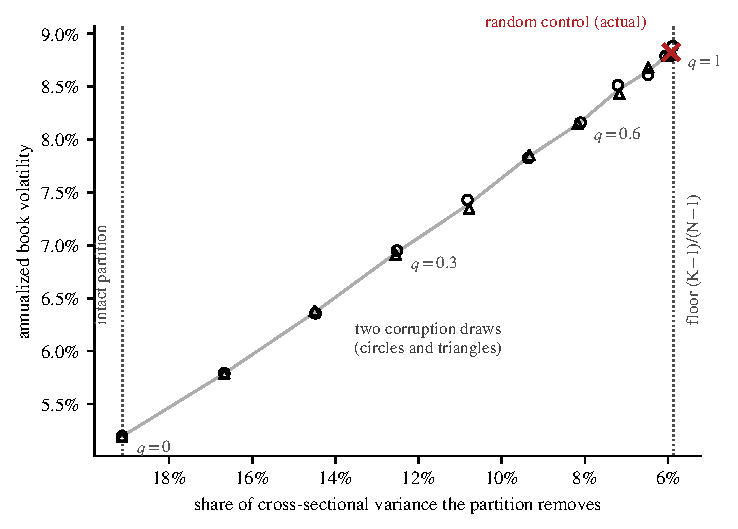
\includegraphics[width=.9\linewidth]{fig_dose}
\caption{Corrupting a real partition, one fraction of labels at a time. This figure plots book volatility against the share of cross-sectional variance the corrupted partition removes. Each point is a full $6{,}913$-day rule-based backtest of the
PCA-loadings partition with a fraction $q$ of each day's labels
redrawn uniformly; two independent corruption draws per $q$ nearly
coincide. The horizontal axis is the share of cross-sectional
variance the corrupted partition removes; the dashed verticals mark
the degrees-of-freedom floor $(\K-1)/(\N-1)$ and the intact partition's
share. The cross is the random control itself.}
\label{fig:dose}
\end{figure}

\subsection{The Estimation Window}
\label{app:window}



Random matrix theory supplies a reason the two clusterizers that gain should be the
sensitive ones: both read individual eigenvectors of the sample
correlation matrix, and at $\N = 500$ a population eigenvalue must exceed $1 + \sqrt{\N/T}$ to be recoverable at all \citep{baik2005phase}. The threshold is $5.9$ at $T = 21$, under which only the market mode survives, against $2.4$ at $T = 252$, under which sector-scale structure does. A rival explanation, however, fits the same six observations, three clusterizers at two windows. The largest gains go to the clusterizers that started lowest, and a regression of the gain on the $21$-day starting level fits with $r = -0.93$. The two explanations make the same prediction on every arm in the sweep. We therefore registered, in advance, three arms on
which they differ by construction, and ran them. Average linkage at
$\K=10$ starts low, so the rival predicts a large gain and the
eigenvector account almost none; the observed gain is $+0.04$. The random
control starts lowest of all, so the rival must predict the largest
gain in the design, while the labels are drawn by a random number
generator that cannot read the window; the observed gain is $-0.11$, negative in four of the five seeds. PCA loadings at $\K=50$ reads eigenvectors, so both accounts predict a gain; the observed gain is $+0.33$. The eigenvector account survives, since it predicts which arms move and in which direction,
and the two arms that use no eigenvector do not move. The account misses the sign of the interaction with $\K$: for PCA loadings the same 60-to-$252$-day move is worth
$+0.27$ at $\K=30$ against $+0.33$ at $\K=50$, so the window effect strengthens as the partition is refined. We have no account of that.

Average linkage peaks at 120 days, mid-sweep; \figref{fig:window_twin} shows the $60$-to-$21$-day step of the same sweep against seed noise. That step shows the account's one exception: complete linkage, which reads the same correlation matrix as average linkage and no eigenvector, loses $0.31$, outside its across-seed band. No $p$-value is quoted for the window responses: a paired test across five fits rests on four degrees of freedom, so each step is judged against its arm's own across-seed band instead.

\begin{figure}[tb]
\centering
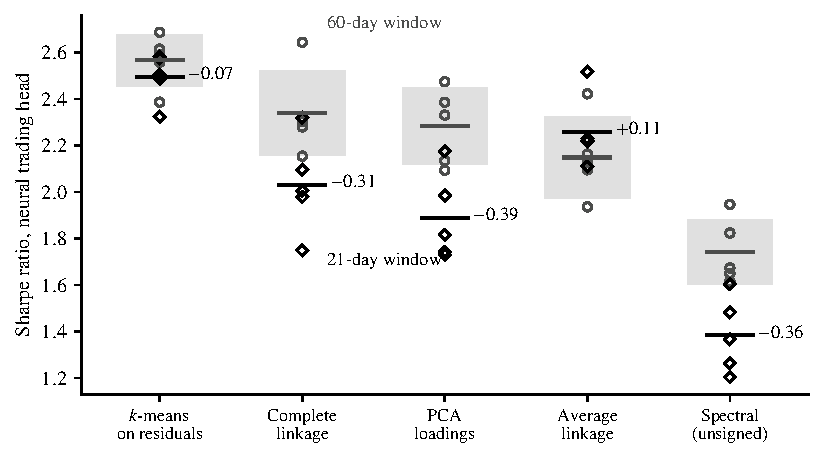
\includegraphics[width=.9\linewidth]{fig_window_twin}
\caption{Changing only the estimation window. This figure plots the per-seed Sharpe ratio at the trained component of the $60$-day arm (circles) against its $21$-day variant (diamonds); the shaded band spans $\pm 1$ across-seed standard deviation of the $60$-day arm, and the horizontal lines are the two windows' seed means. All five $21$-day variants of \appref{app:names} are shown. The two clusterizers that read individual eigenvector coordinates lose $0.39$ and $0.36$, about two and a half times their own band, and complete linkage loses $0.31$; $k$-means on returns moves $-0.07$ and average linkage $+0.11$, both inside their own band.}
\label{fig:window_twin}
\end{figure}

\subsection{Robustness of the Cross-Sectional Projection}
\label{app:lensrobust}

The measurement depends on how many principal components to project
out and which floor to judge the result against. Estimating
the number of factors is a literature of its own \citep{bai2002determining,
onatski2010determining, ahn2013eigenvalue}, and we do not enter it.
At $m = 1, 3, 10$ the $k$-means partition retains $83\%$, $68\%$, $50\%$, and every real partition keeps a strictly positive
excess over its floor at every $m$ tested: the sign of the result is
robust to $m$; the magnitude is not. The floor must also be matched to the partition's own shape. Net of it, retention at five components is $28\%$ to $49\%$ across the 12 clusterizers, and \textsc{gics}, with 10 realized groups on a $322$-name universe, has a floor of $0.028$, not the $0.060$ of \secref{sec:lens}. Against the wrong floor its net retention at 10
components would come out negative, an artifact of over-subtraction. Two details of the protocol qualify these numbers. The retention ratio divides two $R^2$s with different denominators: the share of the post-projection remainder is not a variance decomposition of the original cross-section. The measurement here also counts every group, singletons included, each of which fits its own member exactly. Under the trading convention of \secref{sec:methods}, which deletes singleton members, $k$-means on returns measures $0.264$ on the traded universe with singletons counted (\secref{sec:mechanism}) and $0.216$ without them, against the $0.265$ here.

\subsection{Size of the Spanning Tests}
\label{app:size}

The $t$-statistics of the FF5+MOM block of \tabref{tab:spanning} divide by a Newey--West long-run variance at $21$ lags, and with heavy tails and serial dependence a test of this form can reject more often than its nominal level. We measure its size directly. For each of the 28 books, the null distribution is rebuilt from block-resampled residuals ($21$-day blocks, $5{,}000$ replications per book under each of four independent seeds), with the factor matrix held at its sample values and the betas re-estimated on every draw. The empirical size at nominal $5\%$ is $6.6\%$ pooled across the books and $5.3\%$ to $7.6\%$ book by book. The spread comes from the denominator: dependence cumulated over the $21$ lags is about $1.7$ times as large in the trained books, so the trained books over-reject more. Correcting the size moves the critical value from $1.96$ to $2.2$ in $t$ units even at the worst-behaved book, and the smallest $t$ in that block is $4.1$ ($2.5$ in the block with the reversal factor), so the rejections are not heavy-tail or dependence artifacts.

\subsection{Distance to the Peer Books and Performance}
\label{app:peerdist}

The share of each clusterizer's payoff variance the two peer books explain
runs from $0.52$ to $0.57$, with a positive relation to the clusterizer's Sharpe ratio that falls just short of the $5\%$ level (Spearman $\rho = 0.57$, $p = 0.051$). The overlap between a
clusterizer's positions and the peer books' runs from $0.43$ to $0.48$, or $0.60$ to $0.65$ of what that clusterizer shares with its own refit, with a positive relation to its Sharpe ratio that does not reach significance at the $5\%$ level ($\rho = 0.56$, $p = 0.06$). The two peer books share $0.49$ of their
positions with each other, about as much as either shares with a
clusterizer.

\subsection{Transaction Costs in Detail}
\label{app:costs}

Costs are charged on the positions the runs actually held, so the turnover below is measured from those positions rather than inferred from the payoffs (\appref{app:head}); because the $L^1$ normalization pins the gross book to one (\secref{sec:components}), a position is a share of it. \tabref{tab:costs} reports turnover, the one-way cost at which each book's annual return reaches zero, and net Sharpe ratios at three cost levels. Gross returns run $6.3\%$ to $7.6\%$ a year. At five basis points one-way the same books pay $9.6\%$ to $11.8\%$ a year in cost. Because gross return and cost scale together, the break-even does not depend on leverage.

\begin{table}[tb]
\centering
\caption{Turnover, break-even cost, and net Sharpe ratios}
\label{tab:costs}
\begin{threeparttable}
\small
\setlength{\tabcolsep}{4pt}
\begin{tabular}{@{}lccccccc@{}}
\toprule
& Gross & Return & Turnover & Break-even
& \multicolumn{3}{c}{Net Sharpe ratio} \\
\cmidrule(lr){6-8}
& Sharpe & (\%/yr) & (\%/day) & (bps)
& $1$\,bp & $2$\,bps & $5$\,bps \\
\midrule
12 clusterizers & $1.74$--$2.57$ & $6.62$--$7.60$ & $38.2$--$43.8$ & $3.17$--$3.79$ & $1.20$--$1.86$ & $0.67$--$1.16$ & $-1.24$ to $-0.67$ \\
$\K=1$ & $1.28$ & $6.47$ & $44.6$ & $2.90$ & $0.83$ & $0.38$ & $-0.96$ \\
Random & $1.28$ & $6.25$ & $46.9$ & $2.66$ & $0.79$ & $0.31$ & $-1.15$ \\
\bottomrule
\end{tabular}
\begin{tablenotes}[flushleft]\small
\item \emph{Notes.} This table reports each book's gross Sharpe ratio, annual return, one-way turnover, break-even cost, and net Sharpe ratio at three cost levels. Trained component, five head seeds, each statistic computed per seed and averaged, on the $6{,}913$-day window of \secref{sec:panel} (July 1997 to December 2024). Positions are the weight vectors the runs produced, at gross exposure one. Turnover is one-way, half of
$\sum_i |\Delta w_{it}|$; the break-even and the net columns charge the
full traded notional at the stated one-way rate. Break-even is the one-way rate, in basis points (bps), at which annual return reaches zero. All arms use the common 60-day estimation window of \tabref{tab:methods}; the bands cover the 12 clusterizers, and the two controls are reported on their own rows.
\end{tablenotes}
\end{threeparttable}
\end{table}

The reordering reported in \secref{sec:costs} is not an artifact of the trading head. We run the same measurement on the rule-based component, whose book carries gross exposure two rather than one, and normalize both to the same exposure. Its five-day signal window is rebuilt daily, and its positions correlate with the previous day's at $0.46$ on average across the clusterizers, with $27\%$ of names changing sign. Counted one-way and per unit of gross exposure, the rule-based books turn over $23.1\%$ to $30.8\%$ of their exposure a day against the head's $38.2\%$ to $46.9\%$, and earn $3.9\%$ to $4.6\%$ a year against the head's $6.3\%$ to $7.6\%$. The head trades $1.46$ times as much per unit of exposure and earns $1.63$ times as much, and the two nearly cancel: break-even at the rule-based component is $2.75$ to $3.74$ basis points against $2.66$ to $3.79$ at the trained component. The reordering is sharper without the head: on the rule-based component the two controls finish first and third at five basis points, against ninth and thirteenth at the trained component.

The nearest published comparison runs the other way, and we cannot reconcile the two. \citet{brutti2026orthogonal} report that clustering cuts turnover sharply in their setup, from $87.9\%$ to between $24.2\%$ and $24.4\%$, and charge no costs; our configurations show a far smaller gap, the $\K=1$ control turning over $44.6\%$ against a clustered range of $38.2\%$ to $43.8\%$. Rebalancing frequency is the likely cause (our books are rebuilt every day), but we have not measured it, and we record the divergence as an open question rather than a finding.

Four limitations apply. The cost model is a proportional one-way charge with no market-impact term, and a book rebuilt daily on 500 names is where market impact would be largest. Borrow costs on the short side are not modeled. The panel is US large capitalizations, the most liquid case available, so the break-even here is an upper bound for the same design on a broader universe. Finally, the cost figures are at $\K=30$ only; whether the ordering above survives the sweep of \appref{app:ksweep} is unmeasured.
